\section{Preliminaries}
\label{sec:preliminaries}

\subsection{Stochastic Models}
\label{sec:Stochastic Models}

\begin{definition}[Markov chains]
\label{def:Markov Chains}
A Markov Chain $\mathcal{C}$ is a tuple $(Q, \delta)$ where Q is a finite set of states and 
$\delta: Q \rightarrow \mathbb{D}(Q)$ is a probabilistic transition function, where 
$\mathbb{D}(Q)$ is the set of all probabilistic distribution on a finite set $Q$. A probabilistic distribution on 
$Q$, is a function $f: Q\rightarrow\mathbb{Q}_{\geq0}$ such that $\sum_{q\in Q}f(q)=1$. 
\end{definition}

\noindent
A non-empty finite word $\varrho = p_1p_2...p_n$ over $Q$ is defined as a run of Markov Chain. 
The probability of the run is $\prod_{0\leq i < n}\delta(p_i,p_{i+1})$. 
$\varrho$ reaches $q$, if $q = p_i$ for some $0\leq i\leq n$. 
\newline
\\
The probability of eventually reaching a set of state $T\subseteq Q$ 
in $\mathcal{C}$ starting from $q_0$ can be denoted as $\mathbb{P}^{q_0}_\mathcal{C}[\lozenge T]$. $\lozenge T$ is 
equivalent to $Q\bigcup T$, Q until T. Since not necessary every state in Q is reached before T, 
a set of states $S\subseteq Q$ is defined, where the path until T only consists of these states.
The probability $\mathbb{P}^{q_0}_\mathcal{C}[S\bigcup T]$. If $q_0 \in T$, 
the probability is 1. Otherwise, the probability is calculated as follows: 
\begin{align*}
    \sum\biggl\{ \prod_{0\leq i< n}\delta(q_i,q_{i+1}) ~|~ q_0...q_{n-1}\in (S~\backslash~ T) ~\&~ q_n 
    \in T\ \text{ for } n\geq 1\biggr\}.
\end{align*}

\noindent
If there exists a set $U\subseteq Q$, where all runs from $q_0$ to $T$ reaches, the probability of 
$\mathbb{P}^{q_0}_\mathcal{C}[\lozenge T]$ can be reduced to the following lemma:  

\begin{lemma}
\label{lemma 1}
Consider a Markov Chain $\mathcal{C}=(Q,\delta)$ set of states $U,T\subseteq Q$, and a state $q_0\in Q\backslash U$. 
If $\mathbb{P}^{q_0}_\mathcal{C}[(Q\backslash U)\bigcup T]=0$, then 
\begin{align*}
    \mathbb{P}^{q_0}_\mathcal{C}[\lozenge T] = \sum_{u\in U}\mathbb{P}^{q_0}_\mathcal{C}[(Q\backslash U) \bigcup u]
    \mathbb{P}^{q_0}_\mathcal{C}[\lozenge T]
\end{align*}
\end{lemma}


\begin{definition}[Markov decision processes]
\label{Markov decision processes}
A (finite and discrete-time) Markov decision processes, MDP, $\mathcal{M}$, is a tuple $(Q,A,\delta,T)$ 
where Q is a finite set of states, A a finite set of actions, $\delta: Q \times A \rightarrow \mathbb{D}(Q)$ 
a probabilistic transition function, and $T\subseteq Q$ a set of target state.
\end{definition}

\noindent
The notation for the probability of the state p reaching q with the action a, $\delta(p,a)(q)$ will be changed to 
$\delta(q|p,a)$ for convenience.

\begin{definition}[Strategies]
\label{Strategies}
A (memoryless deterministic) strategy $\sigma$ in an MDP M = $(Q,A,\delta,T)$ is a function $\sigma: Q\rightarrow A$.
\end{definition}

\noindent
\textit{From MDPs to Chains} An MDP $\mathcal{M} = (Q,A,\delta,T)$ and a Markov Chain $M^\sigma = (Q, \mu)$, 
where a strategy $\sigma$ is applied on. $\mu$ is defined as follows: $\mu(q)=\delta(q,\sigma(q))$ for all $q\in Q$.
The probability of q, $\mu(q)$, is the same as $\delta(q,\sigma(q))$, where $\sigma(q)$ gives the action assigned to q. 
\begin{figure}[htb]
	\begin{center}
		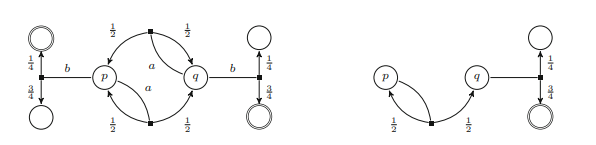
\includegraphics[width=1\linewidth]{pictures/strategies.png}
	\end{center}
	\caption{MDP on the left and 
    on the right a Markov chain induced by the left MDP. \cite{10.1007/978-3-319-89366-2_20}}
	\label{fig:strategies}
\end{figure}

\noindent
The MDP on the left in Figure \ref{fig:strategies} has the actions $\{a, b\}$. The states are shown as circles,
the states with double circles are target states, the squares are distributions. 
The arrows from states to distributions shows which action is used and the arrows from distributions to states are probabilities.
\newline
\\
The strategy $\sigma$ for the right Markov chain maps as follows: $\{p \mapsto a, q \mapsto b\}$ i.e. $\sigma(p) = a, \sigma(q) = b$.
Since the strategy $\sigma$ is applied on the Markov chain, the arrows with actions are removed. 
With the Markov chain, the easier probability to calculate would be $\mathbb{P}^{q}_{\mathcal{M}^\sigma}[\lozenge T] = \frac{3}{4}$.
The probability is written on the arrow from the distributions, after the state q, to the target state.

\subsection{Reachability Games Against Nature}
